\section*{Communication}

For our project, we decided to implement communication with an MQTT (MQ Telemetry Transport) broker, which allows us to send lightweight, continuous messages to our cloud instance.
We used the service shiftr.io, a high-performance broker that easily connects devices to the same network (Figure~\ref{fig:shiftrviz}). \\ \\
To implement communication, we used a MQTT client library in both the Arduino Portenta and our Python backend.
The MQTT client on the Arduino board will send a message after every calibration phase.
The client emits a JSON message on a defined topic, and the Python backend will subscribe to that topic.
When a message is sent from the Arduino, the Python server will receive the message which will then be sent to our ElasticSearch.
\begin{figure}[H]
    \centering
    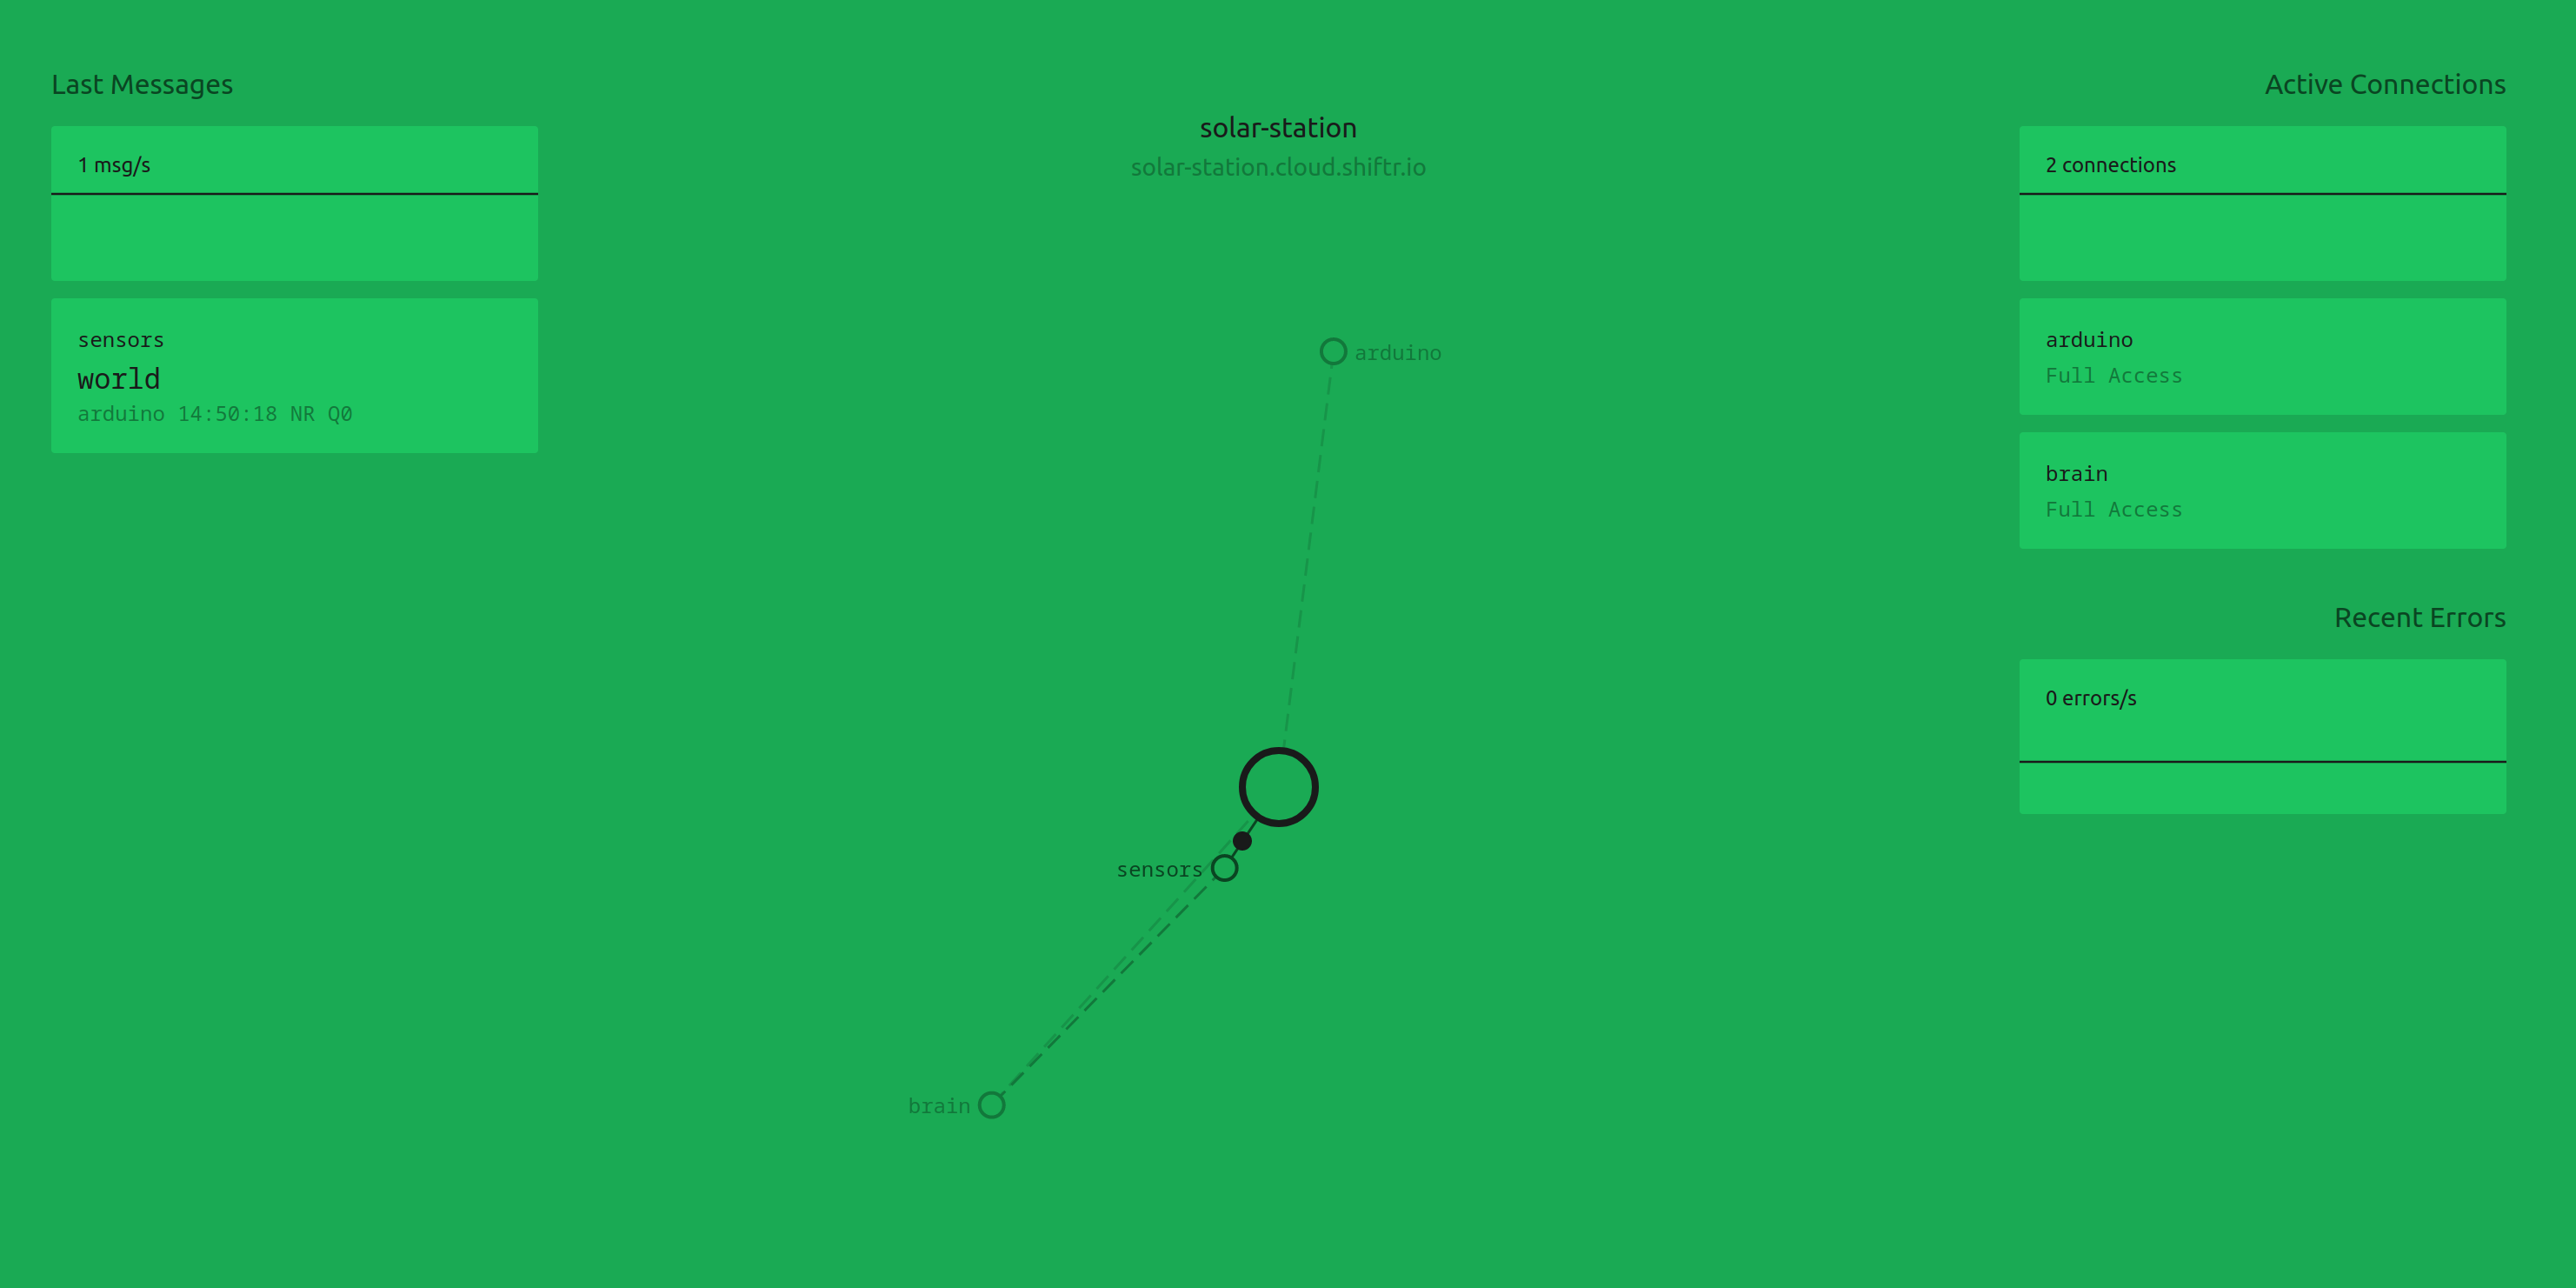
\includegraphics[width=15cm]{../assets/png/shiftr-network}
    \caption{Visualization of our MQTT network through the shiftr.io interface. The "arduino" dot represents our Arduino Portenta device, the "brain" dot represents our Python backend, and the "sensors" dot represents the topic where messages are published.}
    \label{fig:shiftrviz}
\end{figure}
In brief, we used the Arduino WiFi library to connect to the Internet.
We had troubles with USI's WiFi network, as it was necessary to authenticate, so we simply used our mobile hotspots.
We used the Python library Eclipse Paho \footnote{https://pypi.org/project/paho-mqtt} to make our Python client subscribe to the topic, which was trivial.
The respective library on the Arduino side is Arduino MQTT by Joël Gähwiler and contributors \footnote{https://github.com/256dpi/arduino-mqtt}.
